% !TEX encoding = UTF-8
% !TEX TS-program = pdflatex
% !TEX root = ../tesi.tex

%**************************************************************
\chapter{Modello Bradley-Terry per il numero di gol di scarto }
\label{cap:extraDM}
%**************************************************************
\intro{In questo capitolo si illustreranno i risultati ottenuti con il modello Bradley-Terry (\ref{for:4.9}) con una variabile risposta a cinque categorie legate al numero di gol segnati dalle squadre durante le partite.
}
%**************************************************************
\section{Premessa}
Nel Capitolo \ref{cap:risultatiDM} si è sottolineato che i risultati ottenuti non tengono in considerazione le variabili esplicative gol fatti \textsf{GF} e gol subiti \textsf{GA}, a causa della non convergenza del modello. Per poter utilizzare queste due variabili esplicative, su ispirazione del lavoro di ricerca di \textcite{schauberger2017}, si è deciso di cambiare il numero di categorie della variabile risposta \emph{Y} ovvero, di utilizzare cinque categorie invece di tre, in base al numero di gol segnati e subiti, nello specifico:
\begin{equation}
	Res =
	\begin{cases}
		1 & \text{se la squadra in casa batte la squadra ospite con due gol di scarto,}\\
		2 & \text{se la squadra in casa batte la squadra ospite con un gol di scarto,}\\
		3 & \text{se la partita termina con un pareggio,}\\
		4 & \text{se la squadra ospite batte la squadra in casa con un gol di scarto, }\\
		5 & \text{se la squadra ospite batte la squadra in casa con due gol di scarto.}
	\end{cases}       
\end{equation}

\section{Modello Bradley-Terry con Y=5 e Lasso}
I risultati ottenuti dal modello (\ref{for:4.9}) con \emph{Y = 5} sono presentanti nella Figura \ref{tab:BTCL5} e nelle Tabelle \ref{tab:BTCL25} e \ref{tab:BTCL35}.
\begin{sidewaysfigure} 
	\centering
	\begin{center}
		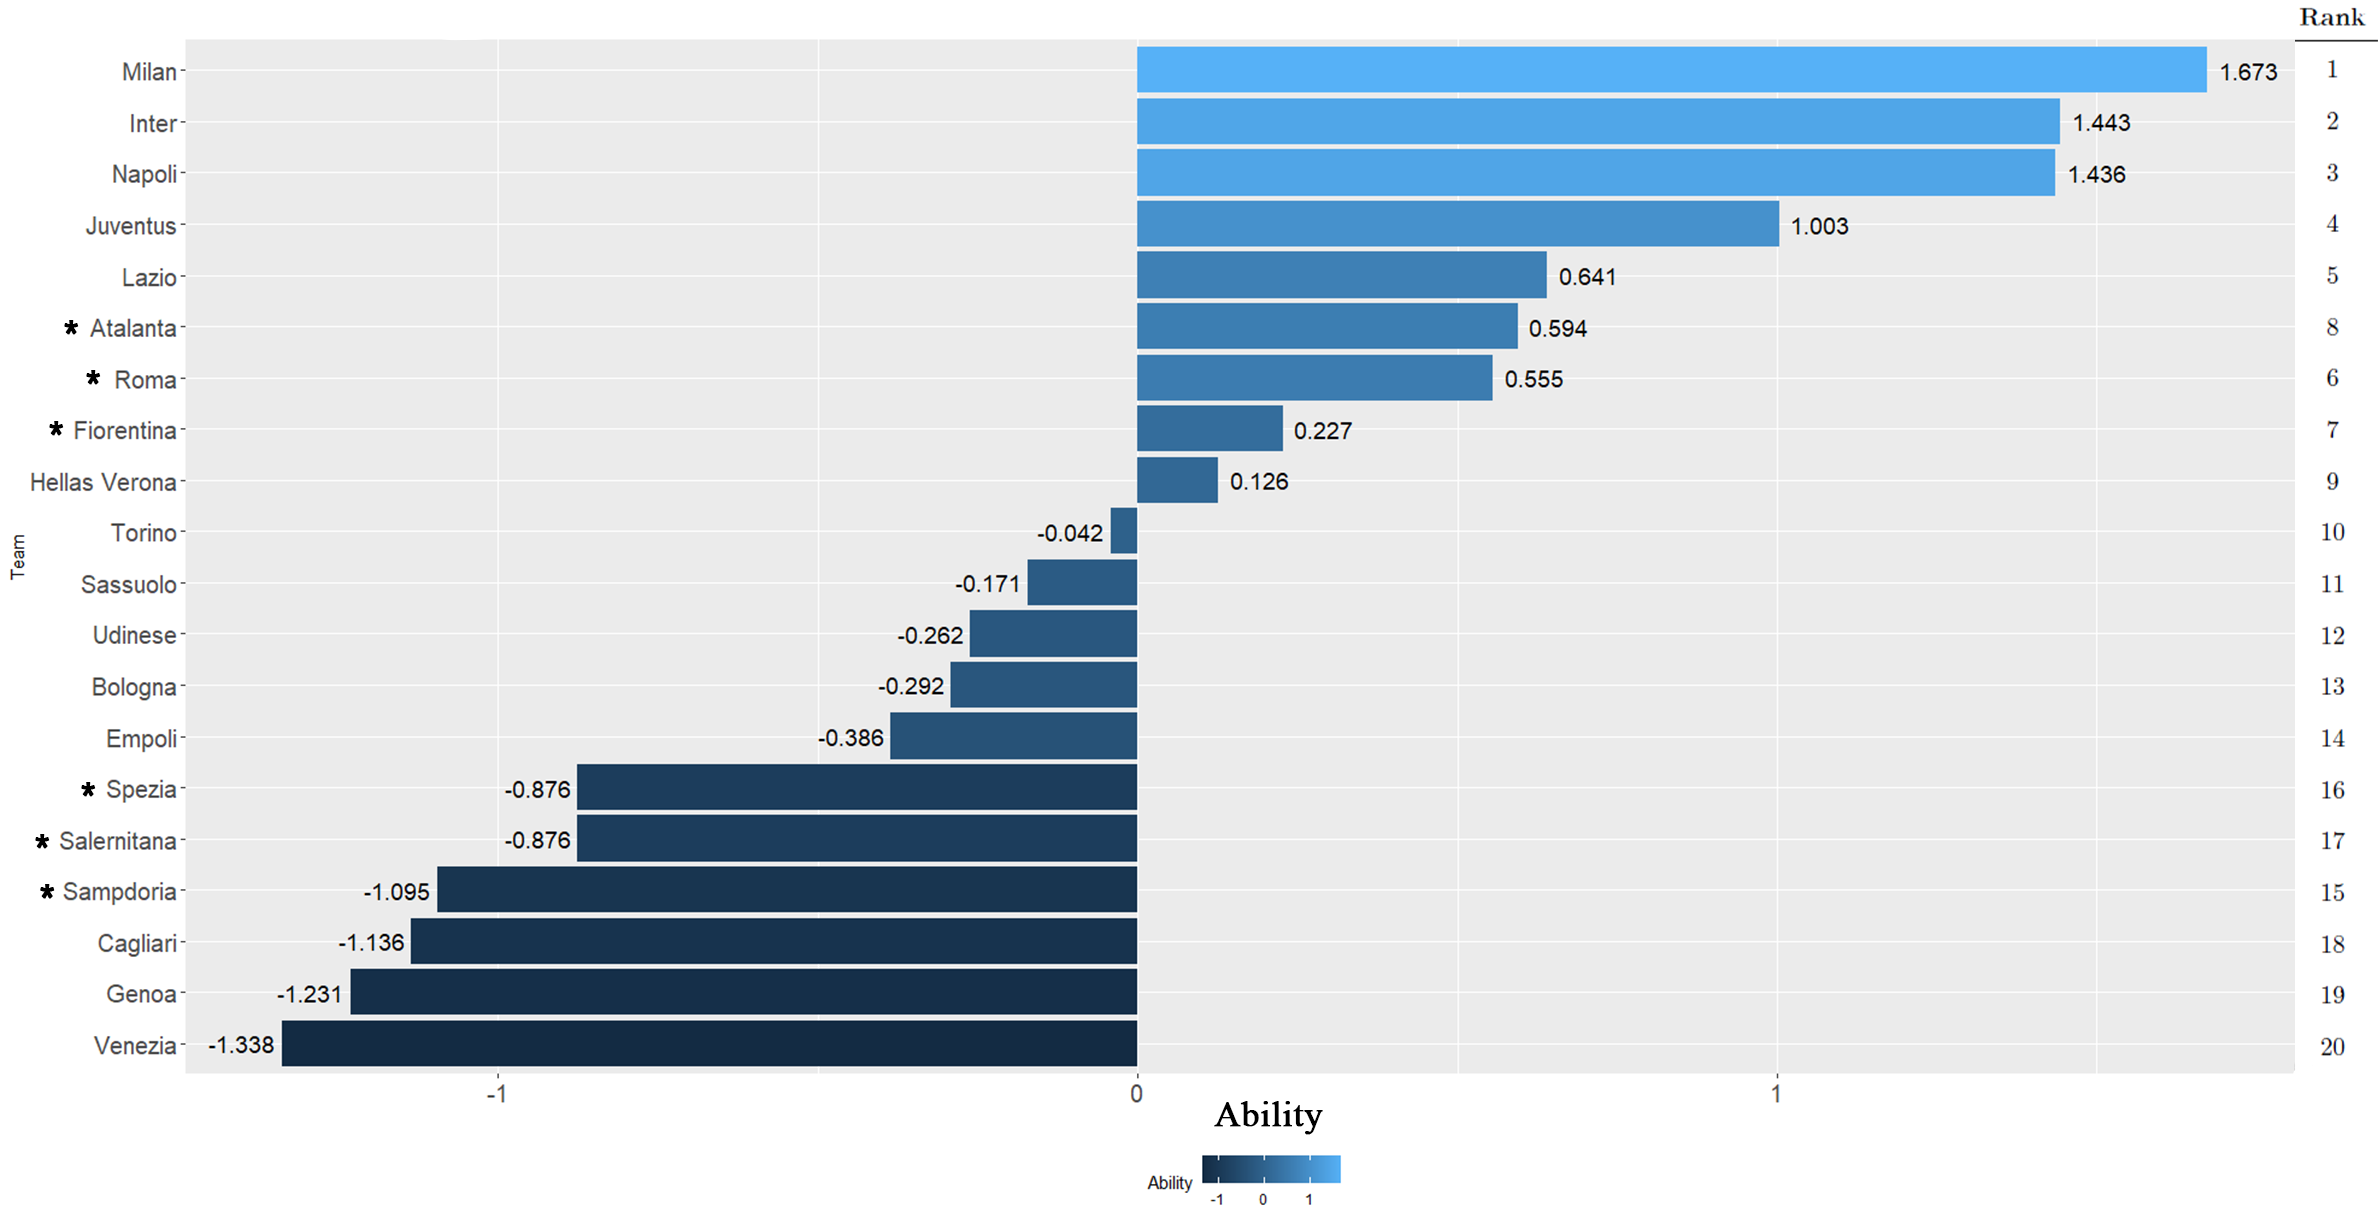
\includegraphics[height=13cm, width=23cm]{rank3.png}
		\caption{Barplot che indica per ogni squadra l'abilità stimata dal modello (\ref{for:4.9}) con \emph{Y = 5}. Viene indicato con un asterisco le squadre con un piazzamento stimato diverso da quello reale anche esso riportato a destra del grafico.} \label{tab:BTCL5} 
	\end{center}
\end{sidewaysfigure}
Nella Figura \ref{tab:BTCL5} si può notare che le stime dell'abilità delle squadre sono molto simile a quelle riportate nella Figura \ref{tab:BTCL}. Infatti, nelle prime e nelle ultime quattro posizioni la stima e il piazzamento rimangono invariati. Cambiano le stime di Atalanta, Lazio e Roma: l'Atalanta aumenta la propria stima e quindi viene ancora più sovrastimata, mentre per Lazio e Roma l'abilità stimata cala. Anche Fiorentina e Hellas Verona hanno un aumento dell'abilità stimata, anche se l'Hellas Verona viene sovrastimata rispetto alla Fiorentina. Infine, anche l'Empoli aumenta la propria abilità stimata, tanto da essere stimato più forte del Bologna.\\
\begin{table}[!htbp]
	
	\renewcommand{\arraystretch}{1.7}
	\centering
	\begin{tabular}{ccp{10cm}}
		\hline	
		
		\textbf{Covariata} & \textbf{Stima} & \textbf{Squadra} \\	
		\hline
		Home & 0.272 & Tutti\\
		Poss & 0.000 & Tutti\\
		Sh & 0.446 & Tutti \\
		SoT & 0.779 & Atalanta, Cagliari, Empoli, Genoa, Verona, Inter, Juventus, Lazio, Milan, Napoli, Roma, Salernitana, Sampdoria, Sassuolo, Spezia, Torino, Venezia\\
		SoT & 0.393 & Fiorentina\\
		SoT & 0.384 & Bologna e Udinese \\
		G/Sh & 1.072 & Tutti \\
		Saves & 0.373 & Tutti \\
		PAtt & 0.000 & Tutti \\
		PCmp\% & 0.000 & Tutti \\
		SPAtt & 0.182 & Napoli \\
		SPAtt & 0.132 & Juventus \\
		SPAtt & 0.000 & Tutti tranne Napoli e Juventus \\
		SPCmp\% & 0.047 & Udinese \\	
		SPCmp\% & 0.000 & Tutti tranne Genoa e Udinese\\ 
		SPCmp\% & -0.030 & Genoa \\	
		MPAtt & 0.000 & Tutti \\ 
		MPCmp\% & -0.188 & Tutti tranne Bologna, Cagliari, Genoa e Spezia \\
		MPCmp\% & -0.201 & Bologna, Cagliari e Spezia \\
		MPCmp\% & -0.262 & Genoa \\
		LPAtt & 0.266 & Lazio \\
		LPAtt & 0.120 & Tutti tranne Lazio \\
		LPCmp\% & 0.236 & Hellas Verona \\
		LPCmp\% & 0.000 & Tutti tranne  Verona \\
		
		\hline
		& &  \\
		
	\end{tabular} \hbox{}
	\caption{Stime delle covariate stimate dal modello (\ref{for:4.9}) con \emph{Y = 5}.} \label{tab:BTCL25} 
	
\end{table}
\begin{table}[!htbp]%
	
	\renewcommand{\arraystretch}{1.7}
	\centering
	\begin{tabular}{ccp{10cm}}
		\hline			
		\textbf{Covariata} & \textbf{Stima} & \textbf{Squadra} \\	
		\hline
		ToDefPen & 0.128 & Tutti \\      
		ToDef3rd & 0.000 & Tutti \\
		ToMid3rd & 0.144 &Tutti\\
		ToAtt3rd & -0.104 & Tutti \\  
		ToAttPen & 0.000 & Tutti tranne Atalanta \\    
		ToAttPen & -0.387 & Atalanta \\ 	     	 
		TotDist & 0.000 & Tutti \\	
		Fls & 0.270 & Sampdoria  \\ 	
		Fls & 0.238 & Bologna  \\
		Fls & 0.000 & Tutti tranne Bologna e Sampdoria  \\
		Fld & 0.130 & Udinese  \\
		Fld & 0.000 & Tutti tranne Udinese \\
		Off & 0.178 & Hellas Verona\\
		Off & -0.030 & Tutti tranne Hellas Verona, Inter e Juventus\\
		Off & -0.034 & Inter e Juventus  \\
		Crs & 0.100 & Torino\\
		Crs & -0.226 & Tutti tranne Milan, Roma, Torino, Atalanta e Napoli\\
		Crs & -0.333 & Milan e Roma\\
		Crs & -0.386 & Napoli\\
		Crs & -0.423 & Atalanta\\
		Int & 0.019 & Tutti\\
		TklWin &  0.083 & Tutti tranne Genoa e Venezia \\ 
		TklWin &  0.000 & Genoa e Venezia \\ 
		Recov &  0.000 & Venezia e Genoa \\ 
		Recov &  -0.044 & Cagliari \\
		Recov &  -0.063 & Tutti tranne Cagliari, Genoa, Udinese e Venezia \\ 
		Recov &  -0.212 & Udinese \\ 
		\hline
		& &  \\
		
	\end{tabular} \hbox{}
	\caption{Stime delle covariate stimate dal modello (\ref{for:4.9}) con \emph{Y = 5}.} \label{tab:BTCL35} 
\end{table}
Le stime dei parametri ottenute sono molto simili alle stime presentate nelle Tabelle \ref{tab:BTCL2} e \ref{tab:BTCL3}. Viene confermata la poca importanza della percentuale dei passaggi completi \texttt{PCmp\%}, del numero di passaggi tentati \texttt{PAtt}, del numero di tocchi nella trequarti di difesa \texttt{ToDefPen} e della distanza percorsa con la palla \texttt{TotDist}.
Anche qui viene confermato, seppur con una leggera diminuzione, il vantaggio nel giocare in casa \texttt{Home} che è pari a 0.272.
Per quanto riguarda il possesso palla \texttt{Poss} viene confermato che per la maggior parte delle squadre non ha alcuna influenza sull'esito della partita. A differenza del modello (\ref{for:4.9}) con \emph{Y = 3}, però, Lazio e Torino non ricevono alcun beneficio.\\
Viene confermata l'associazione positiva con la probabilità di vittoria sia del il numero di tiri \texttt{Sh}, sia del numero di parate \texttt{Saves}. Analogamente, anche la stima per il numero di tiri in porta \texttt{SoT} è fortemente associata all'aumento della probabilità di vittoria. Si segnalano delle variazioni delle stime del parametro \texttt{SoT}. Ora, la maggior parte delle squadre ha una stima del parametro pari a 0.779, ad eccezione di tre squadre. Dalla Figura \ref{fig:sotL5} è possibile individuare tre clusters: il più grande contiene la maggioranza delle squadre, un cluster contiene solo la Fiorentina con un percorso leggermente più basso, un intero cluster contiene Bologna e Udinese.
\begin{figure}[htbp]
	\begin{center}
		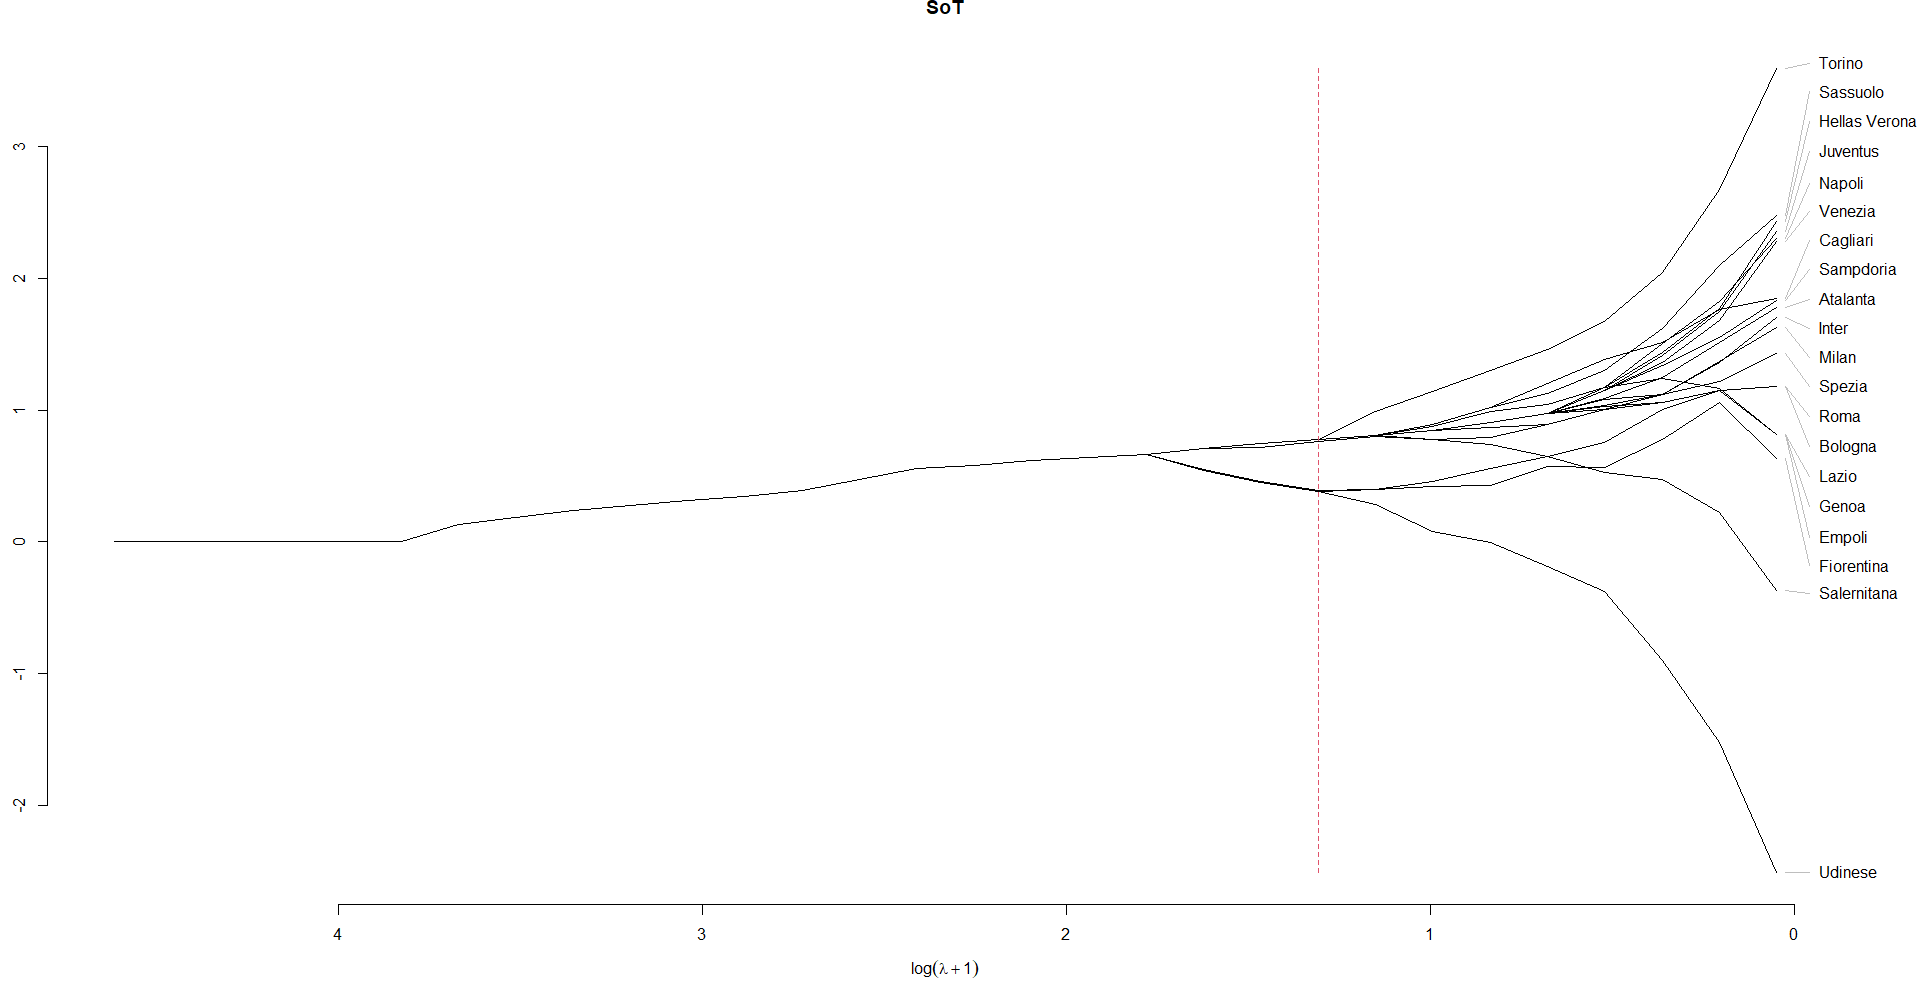
\includegraphics[height=8cm, width=15cm]{sotL5.png}
		\caption{Grafico che riporta l'andamento stimato dal modello (\ref{for:4.9}) con \emph{Y = 5} della stima del numero di tiri in ù+porta per ogni squadra al variare del parametro di tuning $\lambda$. La linea rossa tratteggiata indica il parametro di tuning $\lambda$ ottimo che è stato scelto per ottenere i risultati finali.} \label{fig:sotL5}
	\end{center}
\end{figure}
Si riconferma la variabile esplicativa \texttt{G/Sh} con la maggiormente associata all'esito della partita.\\
Per quanto riguarda le variabili legate ai passaggi non ancora illustrate, viene riconfermato che il numero di passaggi corti tentati \texttt{SPAtt} non risulta essere associato alla probabilità di vittoria per tutte le squadre, ad eccezione di Napoli e Juventus. Nella Figura \ref{fig:spattL5} è possibile notare il cluster con andamento nullo contenente quasi tutte le squadre e più in su i clusters contenenti, rispettivamente, Juventus e Napoli.
\begin{figure}[htbp]
	\begin{center}
		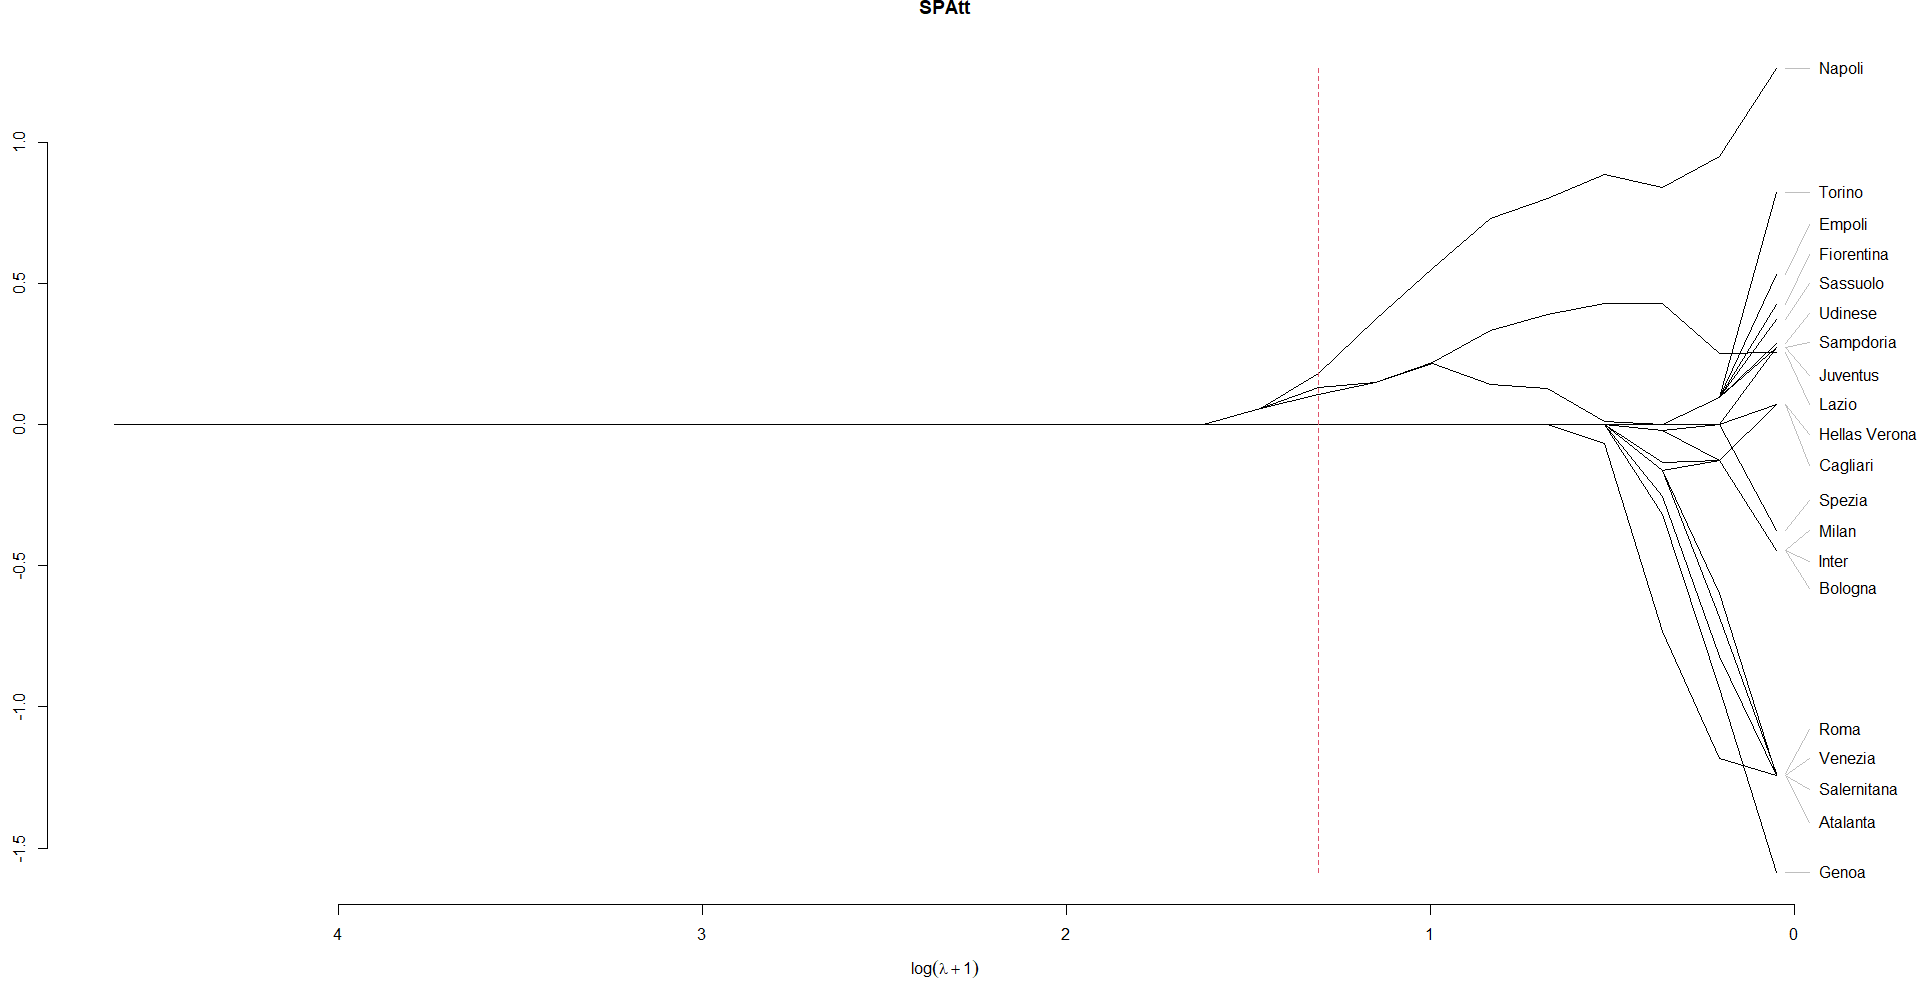
\includegraphics[height=8cm, width=15cm]{spattL5.png}
		\caption{Grafico che riporta l'andamento stimato dal modello (\ref{for:4.9}) con \emph{Y = 5} della stima del numero di passaggi corti tentati per ogni squadra al variare del parametro di tuning $\lambda$. La linea rossa tratteggiata indica il parametro di tuning $\lambda$ ottimo che è stato scelto per ottenere i risultati finali.} \label{fig:spattL5}
	\end{center}
\end{figure}
La percentuale di passaggi corti completati \texttt{SPCmp\%}, invece, ha un importante aumento della stima per il Genoa, mentre solo per l'Udinese è associato un aumento della probabilità di vittoria. Per le restanti squadre, \texttt{SPCmp\%} non ha alcuna associazione con l'esito della partita. Tale risultato è presentato nella Figura \ref{fig:spcmpL5} contenente tre clusters, ognuno per una differente stima.
\begin{figure}[htbp]
	\begin{center}
		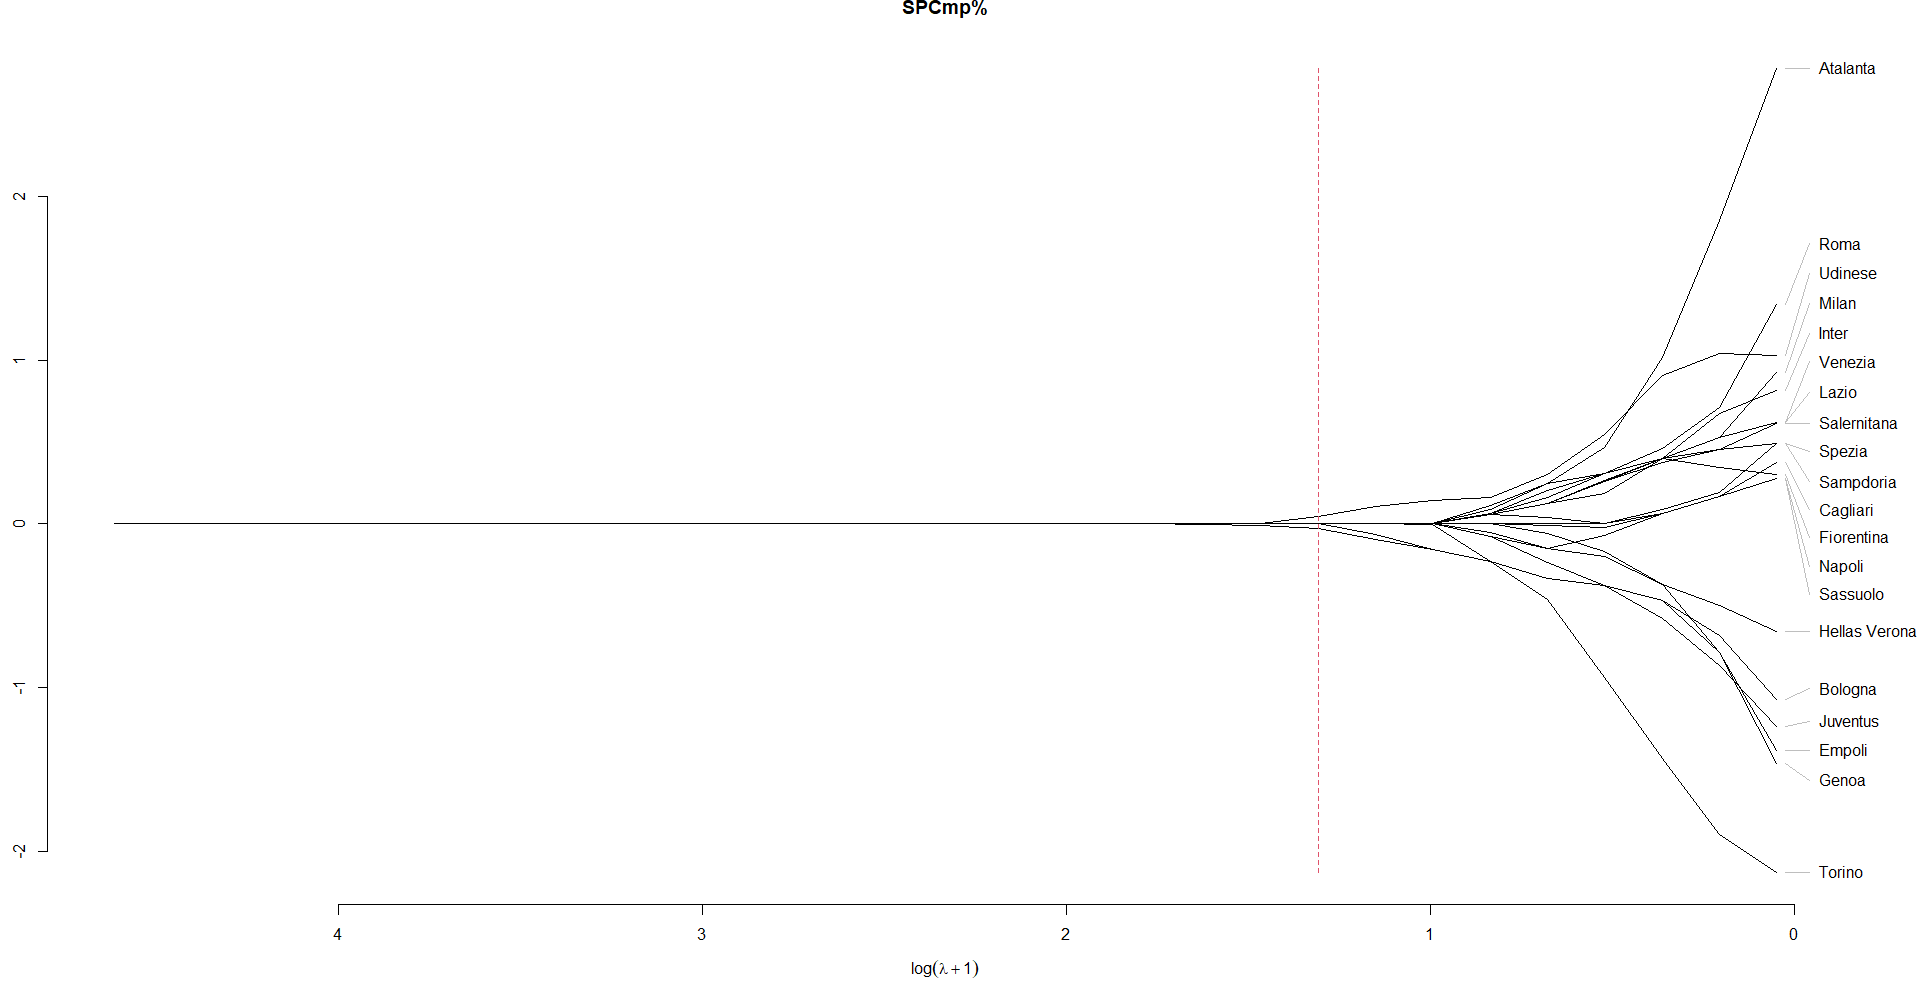
\includegraphics[height=8cm, width=15cm]{spcmpL5.png}
		\caption{Grafico che riporta l'andamento stimato dal modello (\ref{for:4.9}) con \emph{Y = 5} della stima della percentuale di passaggi corti riusciti per ogni squadra al variare del parametro di tuning $\lambda$. La linea rossa tratteggiata indica il parametro di tuning $\lambda$ ottimo che è stato scelto per ottenere i risultati finali.} \label{fig:spcmpL5}
	\end{center}
\end{figure}
Il numero di passaggi medi tentati \texttt{MPAtt} non ha alcuna associazione con l'esito della partita. Rimane ancora associata a una diminuzione della probabilità di vittoria la percentuale di passaggi medi riusciti \texttt{MPCmp\%} per tutte le squadre. Dalla Figura \ref{fig:mpcmpL5} è possibile individuare tre clusters. Il cluster con il percorso meno negativo contiene quasi tutte le squadre, il cluster immediatamente sotto contiene le squadre Bologna, Cagliari e Spezia, mentre il cluster con il percorso associato più negativo contiene il Genoa.
\begin{figure}[]
	\begin{center}
		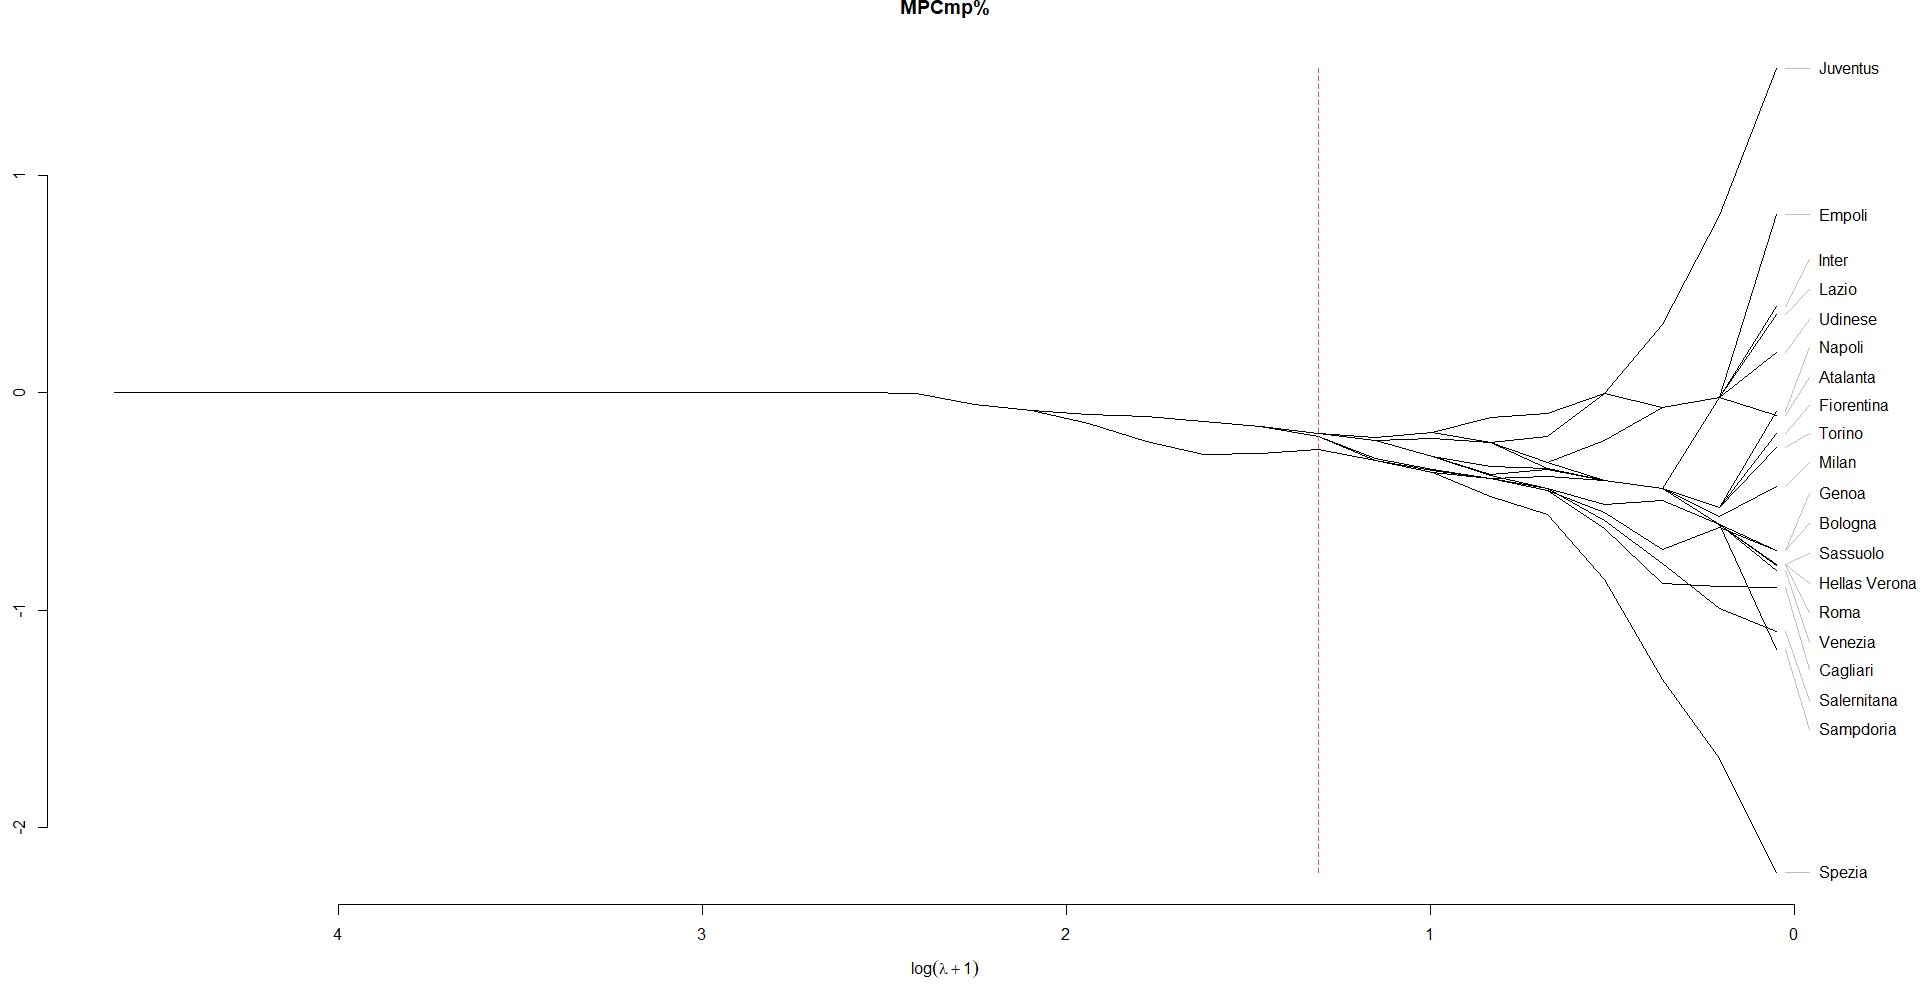
\includegraphics[height=8cm, width=15cm]{mpcmpL5.png}
		\caption{Grafico che riporta l'andamento stimato dal modello (\ref{for:4.9}) con \emph{Y = 5} della stima della percentuale di passaggi medi riusciti per ogni squadra al variare del parametro di tuning $\lambda$. La linea rossa tratteggiata indica il parametro di tuning $\lambda$ ottimo che è stato scelto per ottenere i risultati finali.} \label{fig:mpcmpL5}
	\end{center}
\end{figure}
Per il numero di passaggi lunghi tentati \texttt{LPAtt} c'è un aumento della stima per tutte le squadre, in particolare per la Lazio. Unica variazione che si segnala riguarda la percentuale di passaggi lunghi riusciti \texttt{LPCmp\%} che per il Bologna non è più associata con una diminuzione delle probabilità di vittoria.\\
Per quanto riguarda le variabili legate al possesso, non ci sono rilevanti differenze rispetto alle stime ottenute con il modello (\ref{for:4.9}) con \emph{Y = 3}.\\
Si hanno delle differenze con la stima del numero di falli subiti \texttt{Fls} e fatti \texttt{Fld} rispetto alle stime del modello (\ref{for:4.9}) con \emph{Y = 3}. Infatti, solo per Bologna e Sampdoria \texttt{Fls} è associato a un aumento della probabilità di vittoria, mentre per le restanti squadre non vi è alcuna associazione. Nella Figura \ref{fig:flsL5} è possibile visualizzare l'andamento dei due clusters che contengono, rispettivamente, Bologna e Sampdoria, entrambi con percorsi positivi. È rappresentato anche il cluster contenente quasi tutte le classi, ma con un percorso nullo.
\begin{figure}[htbp]
	\begin{center}
		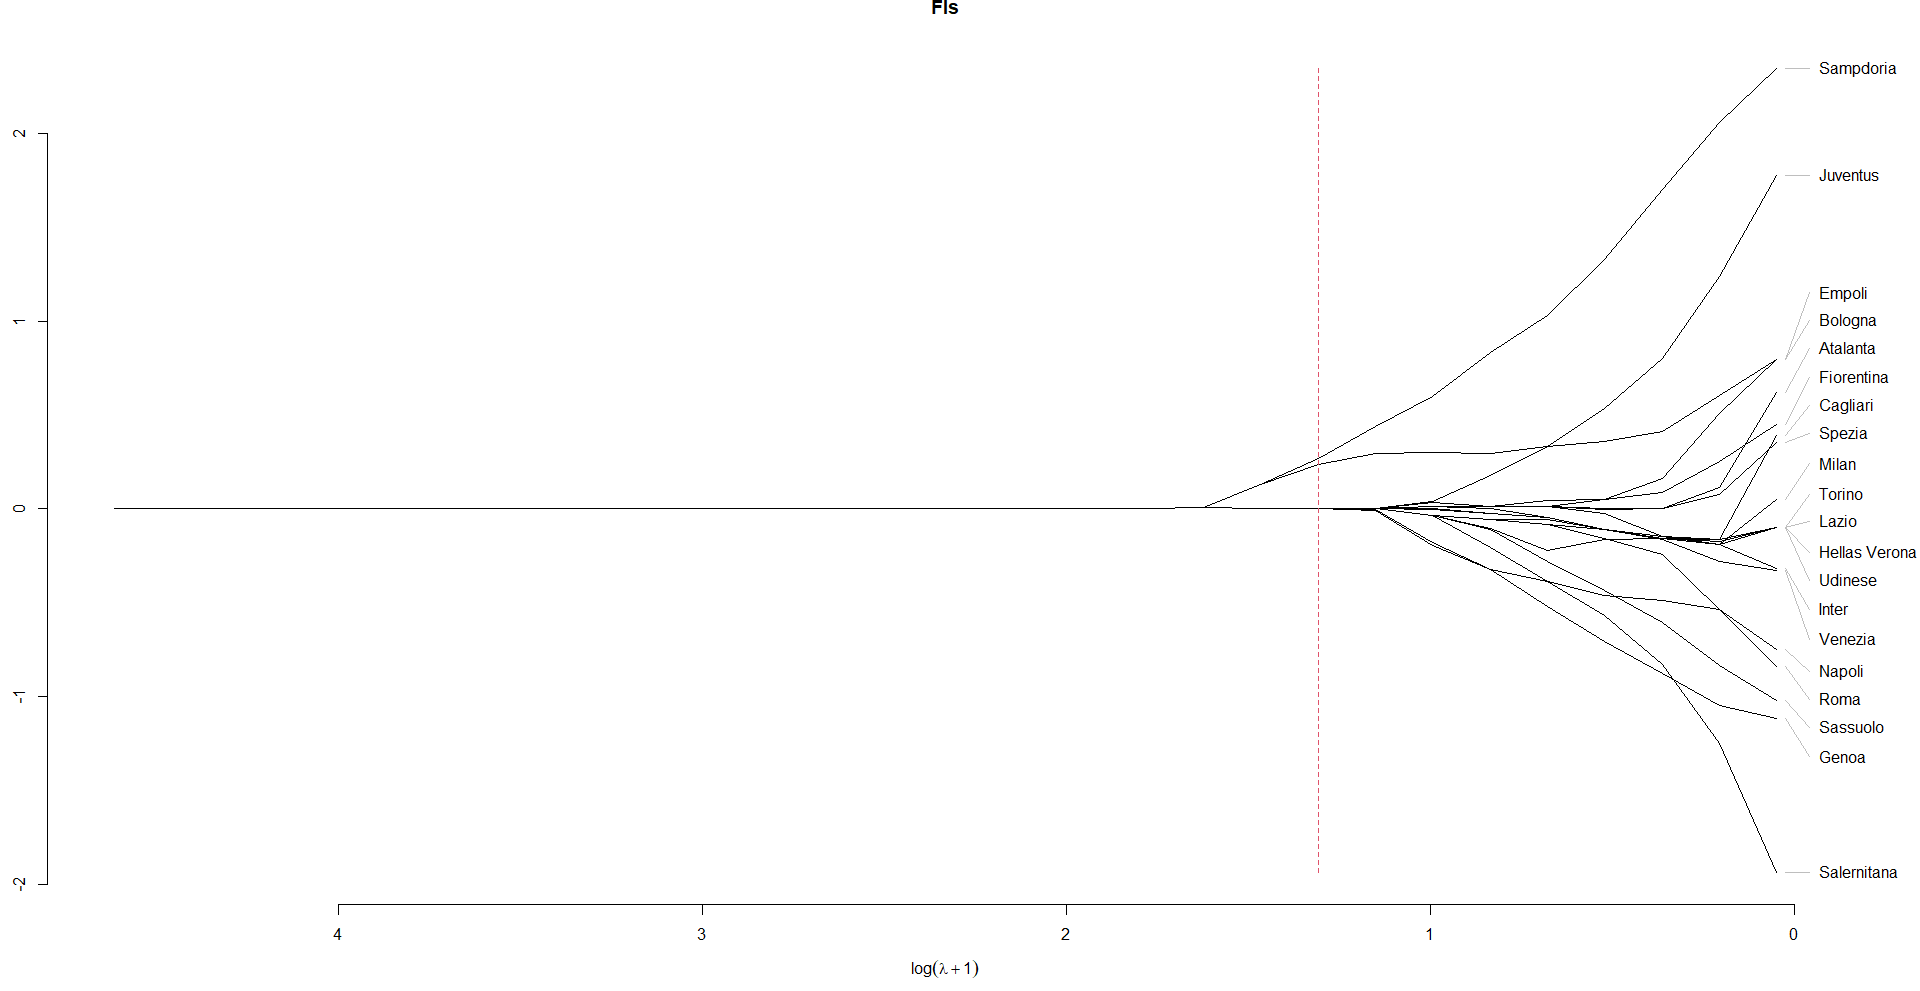
\includegraphics[height=8cm, width=15cm]{flsL5.png}
		\caption{Grafico che riporta l'andamento stimato dal modello (\ref{for:4.9}) con \emph{Y = 5} della stima del numero di falli subiti per ogni squadra al variare del parametro di tuning $\lambda$. La linea rossa tratteggiata indica il parametro di tuning $\lambda$ ottimo che è stato scelto per ottenere i risultati finali.} \label{fig:flsL5}
	\end{center}
\end{figure}
Anche per \texttt{Fld} vi è lo stesso esito con la differenza che, al posto di Bologna e Sampdoria, c'è l'Udinese.\\
Per quanto riguarda il fuorigioco \texttt{Off}, ora solo per l'Hellas Verona vi è una stima positiva. Per tutte le altre squadre la stima è negativa, in particolare per Inter e Juventus.\\
Ancora una volta il numero di cross \texttt{Crs} si conferma associato a una diminuzione della probabilità di vittoria. In questo caso abbiamo una maggior diminuzione per quasi tutte le squadre. Nella Figura \ref{fig:crsL5} è possibile notare il cluster con andamento positivo, il quale contiene il Torino. Sotto al cluster del Torino ci sono quattro cluster tutti associati a percorsi negativi. Il cluster con il percorso meno negativo contiene quasi tutte le squadre. Subito sotto c'è il cluster che contiene Milan e Roma, mentre con un percorso leggermente più negativo, il cluster contenente il Napoli e, infine, con il percorso più negativo, il cluster che contiene l'Atalanta.
\begin{figure}[htbp]
	\begin{center}
		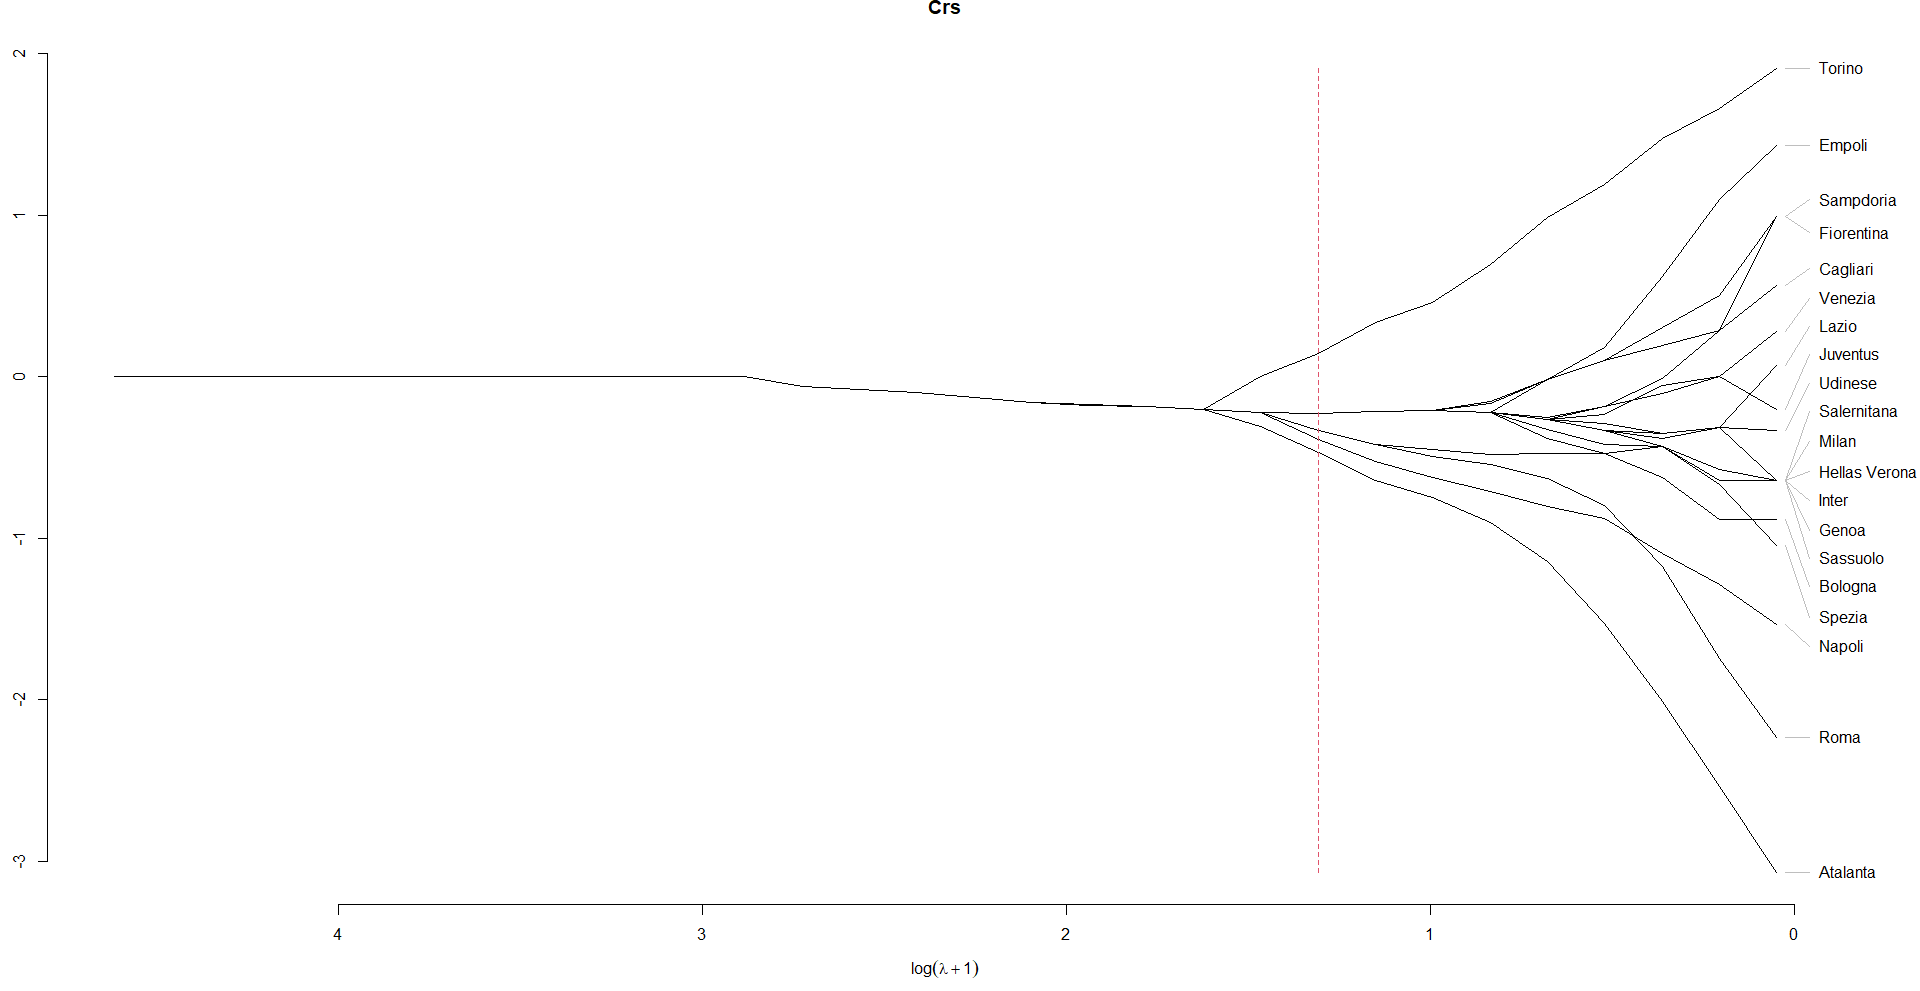
\includegraphics[height=8cm, width=15cm]{crsL5.png}
		\caption{Grafico che riporta l'andamento stimato dal modello (\ref{for:4.9}) con \emph{Y = 5} della stima del numero di cross fatti per ogni squadra al variare del parametro di tuning $\lambda$. La linea rossa tratteggiata indica il parametro di tuning $\lambda$ ottimo che è stato scelto per ottenere i risultati finali.} \label{fig:crsL5}
	\end{center}
\end{figure}
Per quanto riguarda le variabili esplicative difensive, il numero di intercetti \texttt{Int} e il numero di contrasti vinti \texttt{TklWin} sono ancora associati ad un aumento della probabilità di vittoria. Viceversa, il numero di recuperi \texttt{Recov} si associa ad una diminuzione della probabilità di vittoria per tutte le squadre eccetto per Venezia e Genoa, per le quali non vi è alcuna associazione con l'esito della partita. Tale comportamento è mostrato nella Figura \ref{fig:recovL5}.

\begin{figure}[htbp]
	\begin{center}
		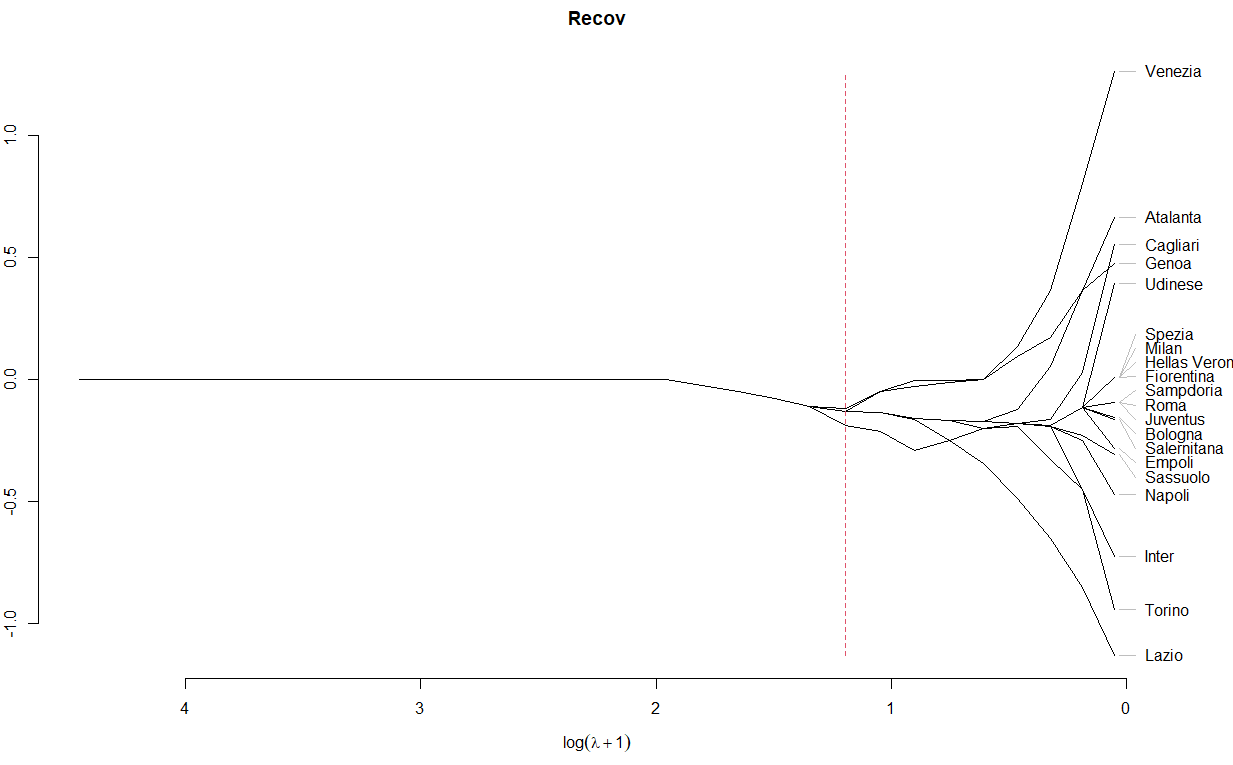
\includegraphics[height=8cm, width=15cm]{recovL.png}
		\caption{Grafico che riporta l'andamento stimato dal modello (\ref{for:4.9}) con \emph{Y = 5} della stima del numero di recuperi per ogni squadra al variare del parametro di tuning $\lambda$. La linea rossa tratteggiata indica il parametro di tuning $\lambda$ ottimo che è stato scelto per ottenere i risultati finali.} \label{fig:recovL5}
	\end{center}
\end{figure}
Ora che \emph{Y = 5} ci sono due soglie in più, per cui la stima delle soglie $\theta_1$, $\theta_2$, $\theta_3$ e $\theta_4$ vale, rispettivamente, -3.114, 3.114, -1.094 e 1.094.\\
Inoltre, i risultati ottenuti sono frutto di un parametro di tuning $\lambda$ pari a 1.308 scelto attraverso la  K-Fold Cross Validation. Nella Figura \ref{fig:lambda3} è mostrato l'andamento delle prestazioni del modello su tutti i valori assunti dal parametro di tuning $\lambda$ durante l'operazione di K-Fold Cross Validation.
\begin{figure}[htbp]
	\begin{center}
		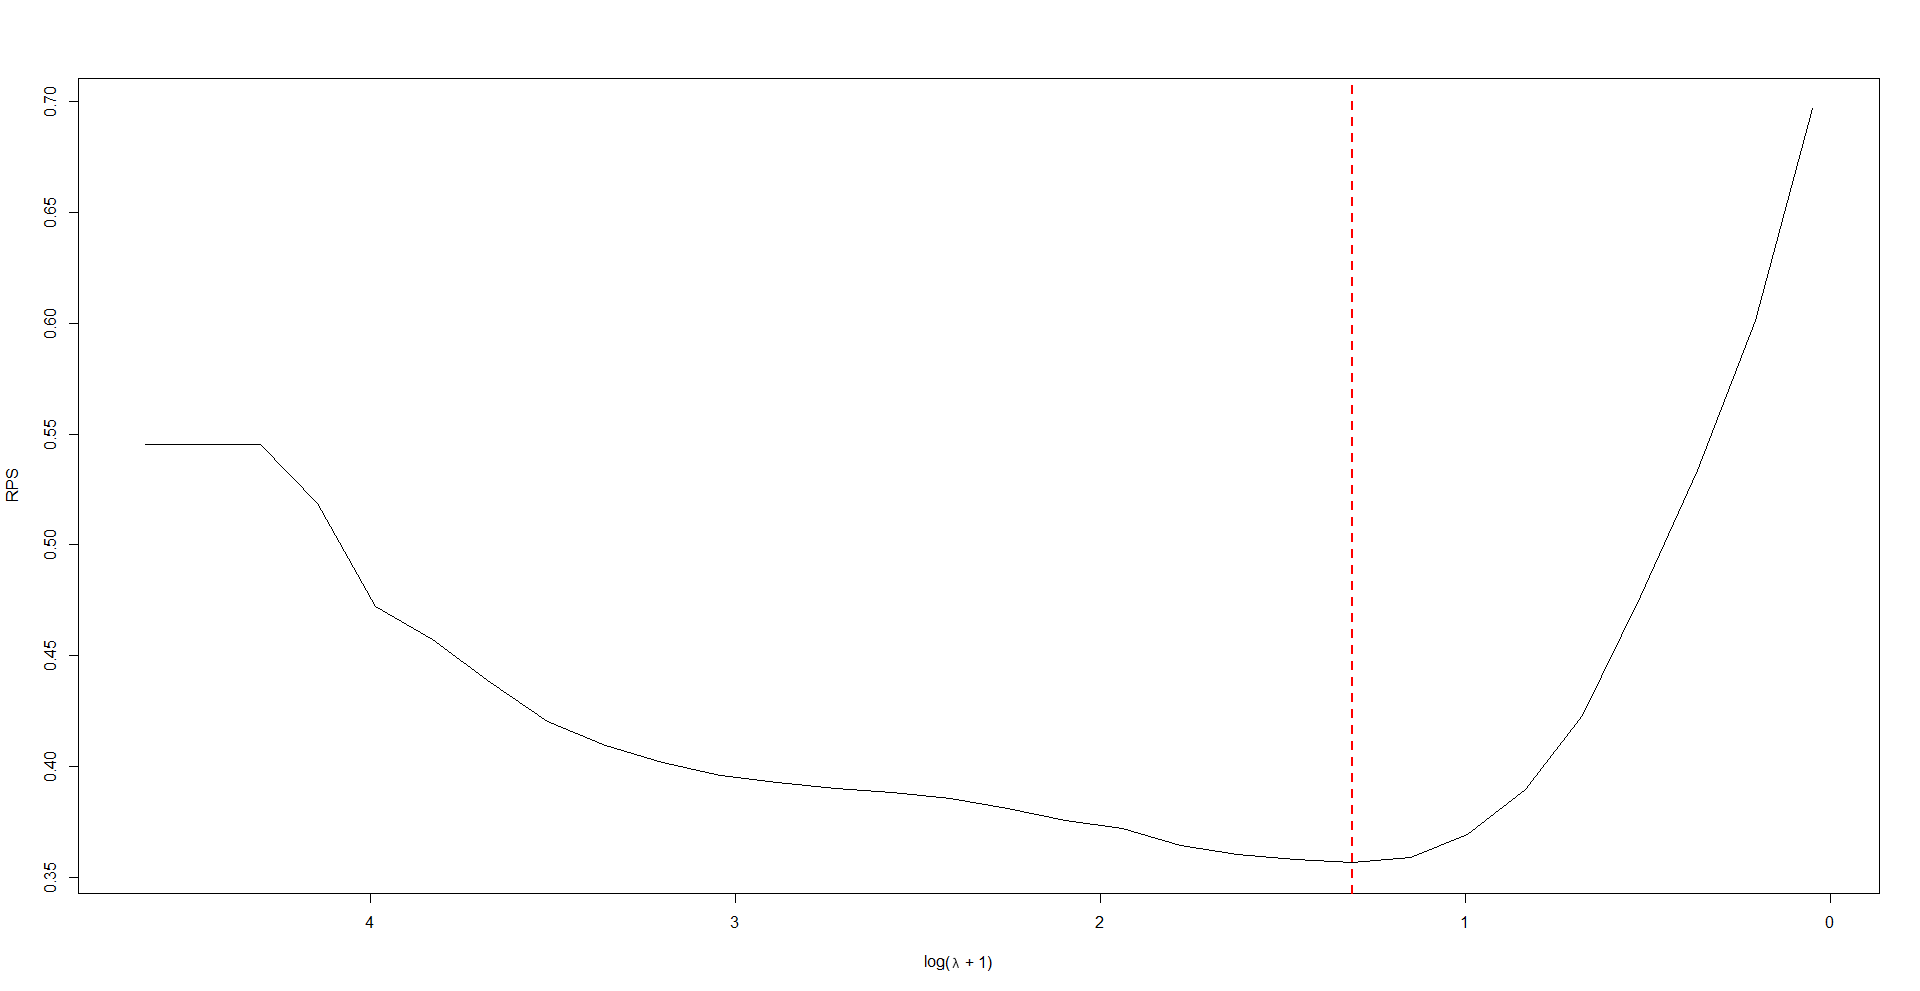
\includegraphics[height=8cm, width=13cm]{CVBTL5.png}
		\caption{Grafico dell'andamento delle prestazioni del modello (\ref{for:4.9}) con \emph{Y = 5}, su tutti i trenta valori assunti dal parametro di tuning, indicato con il simbolo $\lambda$, durante l'applicazione di K-Fold Cross Validation. L'andamento viene valutato in termini di Ranked Probability Score (RPS). La linea rossa tratteggiata indica il parametro di tuning $\lambda$ ottimo da utilizzare.} \label{fig:lambda3}
	\end{center}
\end{figure}
La K-Fold Cross Validation utilizza 10 gruppi (k = 10) e trenta valori diversi per $lambda$. Successivamente, i risultati ottenuti dal modello applicando i trenta diversi valori del parametro di tuning, sono stati confrontati in termini di RPS. Si nota che con il diminuire della penalizzazione il modello registra una RPS che migliora fino a quando la penalizzazione diventa troppo debole, causando un peggioramento delle prestazioni. Si è scelto perciò, il $\lambda$ indicato dalla linea rossa tratteggiata.\\
Per riassumere, si analizzano i percorsi delle norme L2 che rappresentano l'importanza complessiva dei singoli effetti delle covariate. Tali percorsi sono visibili nella Figura \ref{fig:IL52}.
\begin{figure}[]
	\begin{center}
		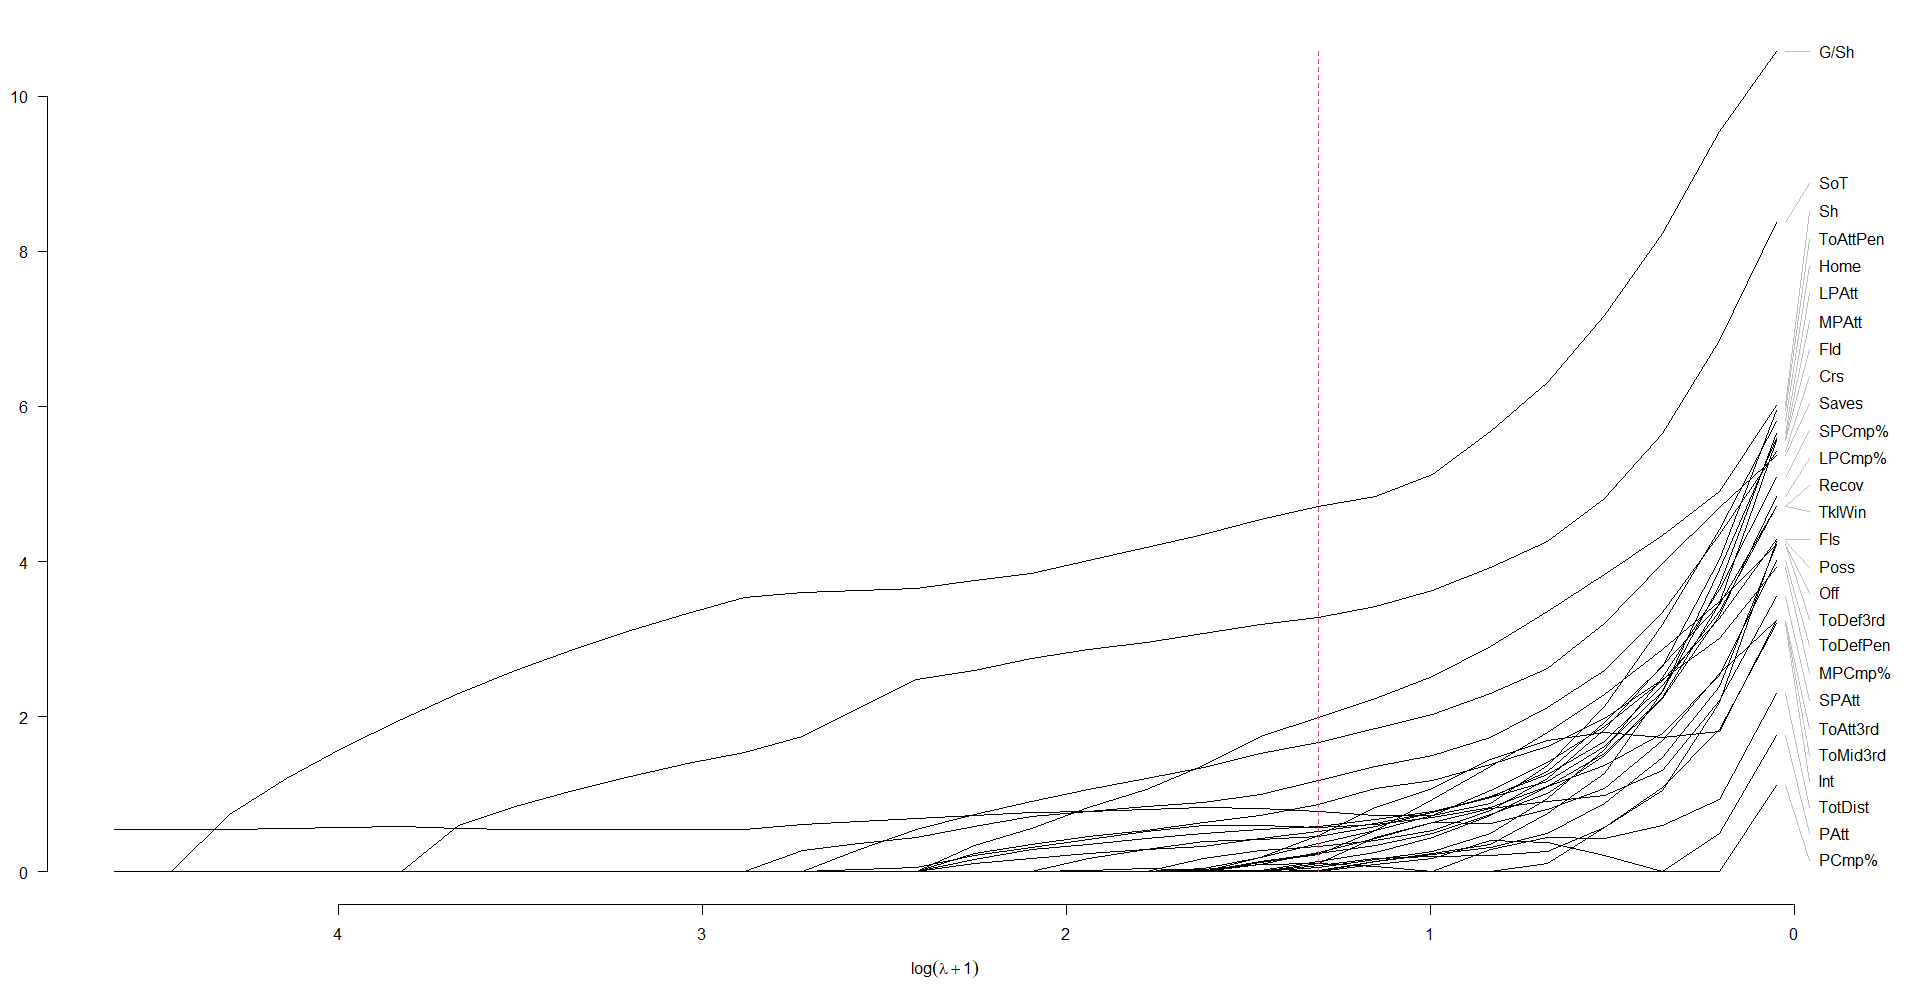
\includegraphics[height=8cm, width=15cm]{IL52.png}
		\caption{Grafico che riporta l'importanza delle covariate rispetto alle norme L2 al variare del parametro di tuning $\lambda$} \label{fig:IL52}
	\end{center}
\end{figure}
Gli andamenti sono molto simili a quelli visti nella Figura \ref{fig:l2BTCL}. Infatti \texttt{G/Sh}, \texttt{SoT} e \texttt{Sh} si confermano ancora fortemente associate all'esito della partita. Analogamente per \texttt{Home}. Si segnala un aumento di importanza per le covariate \texttt{ToAttPen} e \texttt{Recov}, in termini di diminuzione della probabilità di vittoria. Viceversa, si ha un calo d'importanza per \texttt{Saves}, \texttt{Crs}, \texttt{TklWin} e \texttt{Off}. Si riconfermano ancora poco significative le variabili riguardanti i passaggi fatta, eccezione per \texttt{LPAtt}. Anche \texttt{Int} si conferma poco significativo, cosi come \texttt{Poss}.
Pertanto, nel complesso, quanto ricavato del modello (\ref{for:4.9}) con \emph{Y = 3} ora trova conferma anche con la variante \emph{Y = 5}.


\section{Predizioni}
Come fatto nel Capitolo \ref{cap:risultatiDM}, in questa sezione si vuole valutare la prestazione del modello (\ref{for:4.9}) con \emph{Y = 5} nella fase di predizione.\\
Nella Figura \ref{fig:pre2} viene mostrata la classificazione ottenuta perle 80 partite del \emph{test set}.
\begin{figure}[h]
	\begin{center}
		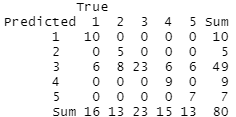
\includegraphics[height = 7cm, width = 13cm]{tabpre2.png}
		\caption{Tabella di confusione che indica le predizioni su 80 partite, fatte dal modello (\ref{for:4.9}) con \emph{Y = 5}. La classe 1 indica la vittoria della squadra in casa con due gol di scarto, la classe 2 indica la vittoria della squadra in casa con un gol di scarto, la classe 3 indica il pareggio tra le due squadre, la classe 4 indica la vittoria della squadra ospite con un gol di scarto e la classe 5 indica la vittoria della squadra ospite con due gol di scarto. Con \textsf{True} si indicano le classificazioni effettive mentre con \textsf{Predicted} le predizioni effettuate.}\label{fig:pre2}
	\end{center}
\end{figure}
Le predizioni ottenute sono buone, con un'accuratezza registrata pari a 0.675. Nella Figura \ref{fig:metrics} vengono mostrate le misurazioni della precisione, della sensibilità e della specificità per ognuna delle cinque categorie registrate sulle predizioni fatte dal modello (\ref{for:4.9}) con \emph{Y = 5}.
\begin{figure}[]
	\begin{center}
		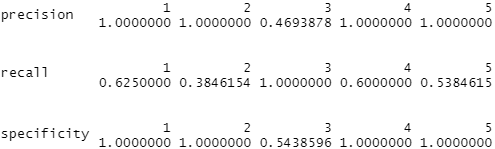
\includegraphics[scale = 0.70]{metrics2.png}
		\caption{Grafico delle misurazioni riguardanti le predizioni fatte dal modello (\ref{for:4.9}) con \emph{Y = 5} su 80 partite. La classe 1 indica la vittoria della squadra in casa con due gol di scarto, la classe 2 indica la vittoria della squadra in casa con un gol di scarto, la classe 3 indica il pareggio tra le due squadre, la classe 4 indica la vittoria della squadra ospite con un gol di scarto e la classe 5 indica la vittoria della squadra ospite con due gol di scarto. Con \textsf{precision} si indicano le misurazioni della precisione per ogni categoria. Con \textsf{recall} si indicano le misurazioni della sensibilità per ogni categoria. Con \textsf{specificity} si indicano le misurazioni della specificità per ogni categoria.}\label{fig:metrics}
	\end{center}
\end{figure}
Le misurazioni ottenute sono buone. In molti casi si registra il miglior risultato possibile, ovvero 1. Nello specifico, analizzando la precisione, si nota che il modello non sbaglia nell’etichettare correttamente tutti le osservazioni, eccetto per il pareggio, per il quale il modello registra una precisione pari a 0.47: delle 49 osservazioni classificate con la classe pareggio solo 23 sono effettivamente della classe pareggio. Tuttavia, analizzando la sensibilità si scopre che, nonostante vengono etichettate erroneamente molte osservazioni con la classe pareggio, sono state identificate tutte le osservazioni di classe pareggio. Ovviamente questo va a scapito delle prestazioni della sensibilità sulle altre classi. Infatti, la sensibilità nella classe vittoria della squadra in casa con un gol di scarto è pari a 0.38: solo cinque su otto osservazioni vengono identificate correttamente appartenenti a questa classe. Analogamente anche per le altre classi si ha un calo nella sensibilità. Tuttavia, le misurazioni ottenute sono discrete. Per quanto riguarda la specificità, analogamente alla precisione, per tutte le classi si registra il miglior risultato possibili eccetto per la classe pareggio dove la specificità è pari a 0.54, poiché 26 osservazioni vengono erroneamente classificate con la classe pareggio.


